\chapter*{\textit{Interlude: Transitioning to Development}} \label{sec:interlude}
\addcontentsline{toc}{chapter}{Interlude: Transitioning to Development}

% TODO: Convert this into introductions for the other parts

Up until this point, the project has been focused on experimentation, research, and prototyping. Chapters \ref{sec:heatpumpcollection} through \ref{sec:simulationprototype} have identified key use cases, requirements, and architectures for processing live data. 
\Cref{sec:heatpumpcollection} identified that while data collection is straightforward, there are limitations to the data that can be collected. Often, custom logic for inference or sensor fusion will be required. \Cref{sec:architectureresearch} tested the conclusions from the literature review, concluding that IDAES is capable of supporting dynamic modelling, surrogate modelling, optimisation, and control, but that these features mean different things in the context of live data processing compared to offline simulation. \Cref{sec:simulationprototype} demonstrated that the Ahuora Simulation Platform could be integrated with a real-time data processing system for steady-state modelling with relatively little effort, as long as there was a standardised API, and provided techniques to do so. However, much more complexity arises when combining all these concepts together, and when balancing the needs of the engineer's workflow with the operator's workflow.

The best way to prove the efficacy of this system is to start building it. Even though the perfect architecture has not yet been found, it is quicker to build a system and iterate on it than to try to design the perfect system from the start. The following chapters are focused on developing the Ahuora Simulation Platform to support live data processing, and iteratively testing these developments on the Heat Pump Dryer Model.

The research conducted so far has provided the context required to build a high-level roadmap of future development. This is shown in \cref{fig:development_flowchart}, where the development is broken down into phases. Each phase is broken down into subtasks, identifiying the key challenges to overcome.
Phase 1 provides the core functionality: ingesting data, solving the simulation, and displaying the results. This is the minimum viable product, and constitutes the main objective of this project. Phase 2 adds support for physics based modelling, optimisation, and control. The key challenges anticipated, including specifying input of the the time domain, holdup, and visualisation, come from the research conducted in \cref{sec:dynamicmodelling}. Likewise, the key challenges from optimisation and control originate from the research in \cref{sec:optimisationcontrol}. Based on research from the literature review and \cref{sec:surrogatemodelling} surrogate modelling moves beyond IDAES alone, and may also include online learning methods, specified in the figure as ``Live Surrogate Modelling''. This was seperated out as Phase 3, because it is a wider goal, and less defined at this stage. 

Phase 2 and 3 will not be developed in this project, but the long-term roadmap is a key research outcome in itself. This proves that development has been done in an engineering context, with a clear understanding of future requirements and an anticipation of further work.

% Todo: Put this in the proposed architecture section.
\begin{landscape}
    \begin{figure}
        \centering
        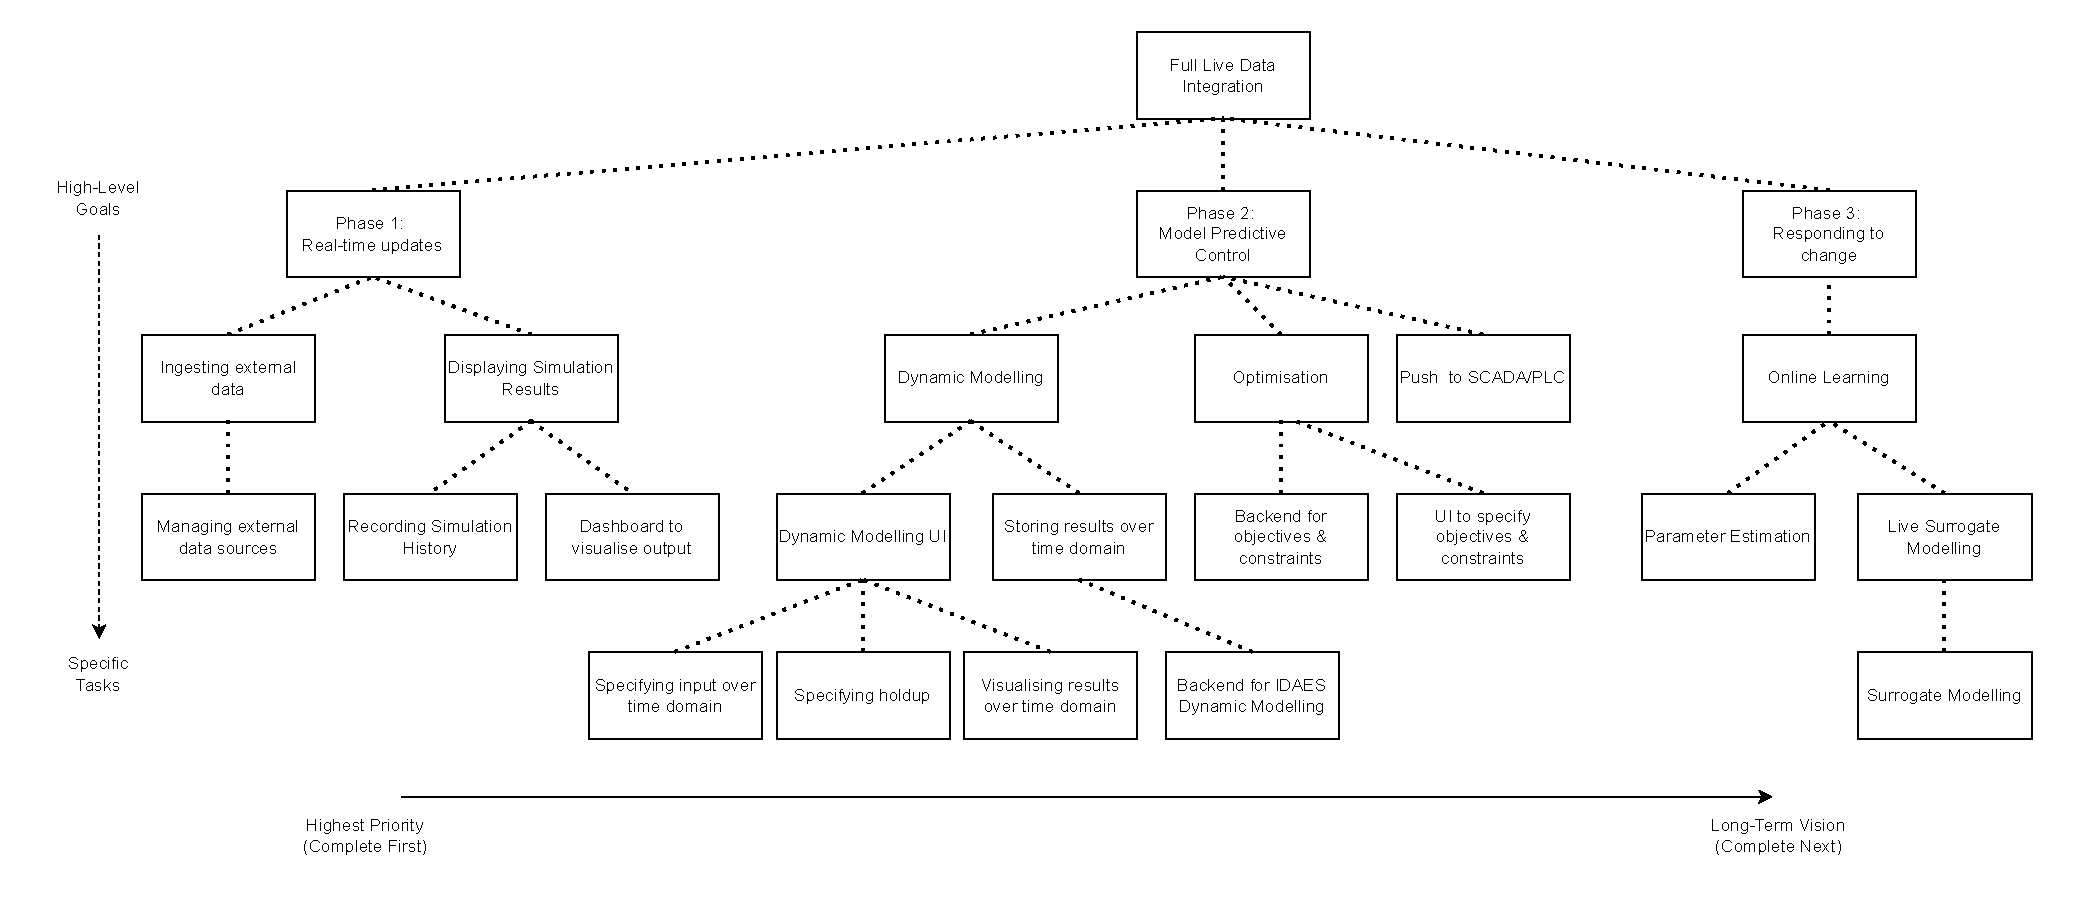
\includegraphics[width=1.5\textwidth]{roadmap.pdf}
        \caption{Roadmap of future development, broken down into tasks. This extends beyond the scope of this project, into the broader vision of the Ahuora Digital Twin Platform. Each task is a key milestone in creating an industry-ready live data processing platform.}
        \label{fig:development_flowchart}
    \end{figure}
\end{landscape}
